% THIS IS SIGPROC-SP.TEX - VERSION 3.1
% WORKS WITH V3.2SP OF ACM_PROC_ARTICLE-SP.CLS
% APRIL 2009
%
% It is an example file showing how to use the 'acm_proc_article-sp.cls' V3.2SP
% LaTeX2e document class file for Conference Proceedings submissions.
% ----------------------------------------------------------------------------------------------------------------
% This .tex file (and associated .cls V3.2SP) *DOES NOT* produce:
%       1) The Permission Statement
%       2) The Conference (location) Info information
%       3) The Copyright Line with ACM data
%       4) Page numbering
% ---------------------------------------------------------------------------------------------------------------
% It is an example which *does* use the .bib file (from which the .bbl file
% is produced).
% REMEMBER HOWEVER: After having produced the .bbl file,
% and prior to final submission,
% you need to 'insert'  your .bbl file into your source .tex file so as to provide
% ONE 'self-contained' source file.
%
% Questions regarding SIGS should be sent to
% Adrienne Griscti ---> griscti@acm.org
%
% Questions/suggestions regarding the guidelines, .tex and .cls files, etc. to
% Gerald Murray ---> murray@hq.acm.org
%
% For tracking purposes - this is V3.1SP - APRIL 2009

\documentclass{acm_proc_article-sp}
\graphicspath{ {./images/} }
\usepackage{subcaption}

\begin{document}

\title{Forecasting building occupancy: A comparative study of approaches}
%\subtitle{[Extended Abstract]
%\titlenote{A full version of this paper is available as
%\textit{Author's Guide to Preparing ACM SIG Proceedings Using
%\LaTeX$2_\epsilon$\ and BibTeX} at
%\texttt{www.acm.org/eaddress.htm}}}
%
% You need the command \numberofauthors to handle the 'placement
% and alignment' of the authors beneath the title.
%
% For aesthetic reasons, we recommend 'three authors at a time'
% i.e. three 'name/affiliation blocks' be placed beneath the title.
%
% NOTE: You are NOT restricted in how many 'rows' of
% "name/affiliations" may appear. We just ask that you restrict
% the number of 'columns' to three.
%
% Because of the available 'opening page real-estate'
% we ask you to refrain from putting more than six authors
% (two rows with three columns) beneath the article title.
% More than six makes the first-page appear very cluttered indeed.
%
% Use the \alignauthor commands to handle the names
% and affiliations for an 'aesthetic maximum' of six authors.
% Add names, affiliations, addresses for
% the seventh etc. author(s) as the argument for the
% \additionalauthors command.
% These 'additional authors' will be output/set for you
% without further effort on your part as the last section in
% the body of your article BEFORE References or any Appendices.

\numberofauthors{2} %  in this sample file, there are a *total*
% of EIGHT authors. SIX appear on the 'first-page' (for formatting
% reasons) and the remaining two appear in the \additionalauthors section.
%
\author{
% You can go ahead and credit any number of authors here,
% e.g. one 'row of three' or two rows (consisting of one row of three
% and a second row of one, two or three).
%
% The command \alignauthor (no curly braces needed) should
% precede each author name, affiliation/snail-mail address and
% e-mail address. Additionally, tag each line of
% affiliation/address with \affaddr, and tag the
% e-mail address with \email.
%
% 1st. author
\alignauthor
James Howard\\\
       \affaddr{Colorado School of Mines}\\
       \affaddr{1500 Illinois St.}\\
       \affaddr{Golden, CO 80401}\\
       \email{jahoward@mines.edu}
% 2nd. author
\alignauthor
William Hoff\\\
       \affaddr{Colorado School of Mines}\\
       \affaddr{1500 Illinois St.}\\
       \affaddr{Golden, CO 80401}\\
       \email{whoff@mines.edu}
}

\date{17 May 2013}


\maketitle
\begin{abstract}
Occupancy knowledge of a building can lead to significant improvements in smart heating and cooling systems.  In this work we gather occupancy information using passive infrared motion sensors densely placed throughout an office building and a classroom building.  

We then compare a number of forecasting algorithms including a Bayesian combined predictor made up of other simpler algorithms on these datasets.  Because the buildings have such different occupancy profiles we compare our algorithms on each dataset to get a better idea of what forecasting algorithm is most ideal for a given set of conditions.  
\end{abstract}

% A category with the (minimum) three required fields
%\category{H.4}{Information Systems Applications}{Miscellaneous}
%A category including the fourth, optional field follows...
%\category{D.2.8}{Software Engineering}{Metrics}[complexity measures, performance measures]

%\terms{Theory}

%\keywords{ACM proceedings, \LaTeX, text tagging} % NOT required for Proceedings

\section{Introduction}

According to the U.S. Department of Energy energy for heating and cooling accounts for approximately 35 - 45\% \cite{DOE2010} of the total expenditure within a building. With such a large investment of energy being used to regulate the temperature of a building, any possible areas of improvement in this area are heavily sought after.   Knowledge of occupancy of people within a building are an important component to intelligent heating and air condition systems.  True levels of occupancy are rarely known and as a results most buildings instead rely on existing systems such as carbon dioxide sensors or motion activated lights.  

In this paper we explore the forecasting accuracy of multiple common time series forecasting models as well as a Bayesian combined predictor trained using those models on real world occupancy data using a number of forecasting measurement metrics.  Occupancy data is difficult to acquire and accurate ground truth values are rare as most buildings do not have sufficient infrastructure to properly sense people accurately throughout the building.  Thus there has been considerable work in generating simulated models of occupancy \cite{PAGE2008, GOLDSTEIN2010}.  These simulations often involve agent based models where the concern is more with the accuracy of the models occupancy at any given time instead of the model's forecasting abilities.   Agent based models also tend not to scale well to large buildings where the where large numbers of agents, rooms and interactions lead to non-trivial solutions. A number of other researchers have created local wireless network occupancy sensing devices using a combination of sensors.  

To acquire real occupancy estimates without simulation there have been multiple systems using a combination of simple sensors and wireless motes.  Agarwal, et. al \cite{Agarwal2010} has created motes using a combination of an IR sensors reed switch place on a door to determine the likelihood that a room is occupied.  Mamidi \cite{Mamidi2012} and the University of Southern California have developed a building-level energy management system using a combination of motion detectors and environmental sensors.  Ground truth was collected and used as the basis for target values which were then run through a machine learning algorithm to accurately estimate occupancy.  In both of these instances the occupancy estimation was limited to a small set of rooms only.

Our occupancy estimates are instead derived from a set of infrared sensors densely placed around a building.  The data is collected from two different types of buildings, one is an office building, the other a classroom and research building with different schedules of levels occupancy.  We also are not concerned only with short term forecasting as pre-heating and pre-cooling building control systems accept forecasts up to one day into the future \cite{Ma2010}.  Thus our analysis will be on forecasts from 10 minutes to hours into the future.  We believe that this work will lead researchers to have a better idea of what forecasting algorithms will perform best under the specific conditions of our buildings.  

The remainder of the paper is laid out as follows: Section 2 introduces the datasets and gives a brief description of the data collection method and the types of buildings from which the data was generated.  Section 3 discusses the forecasting algorithms along and any specific considerations we had to take to apply that algorithm to our problem.  In section 4 we discuss the metrics we will use to analyze the data and show the results of our forecasts.  Finally the paper concludes with a discussion of our conclusions in section 5.

\begin{figure*}[t!]
\centering
\begin{subfigure}{.45\textwidth}
  \centering
  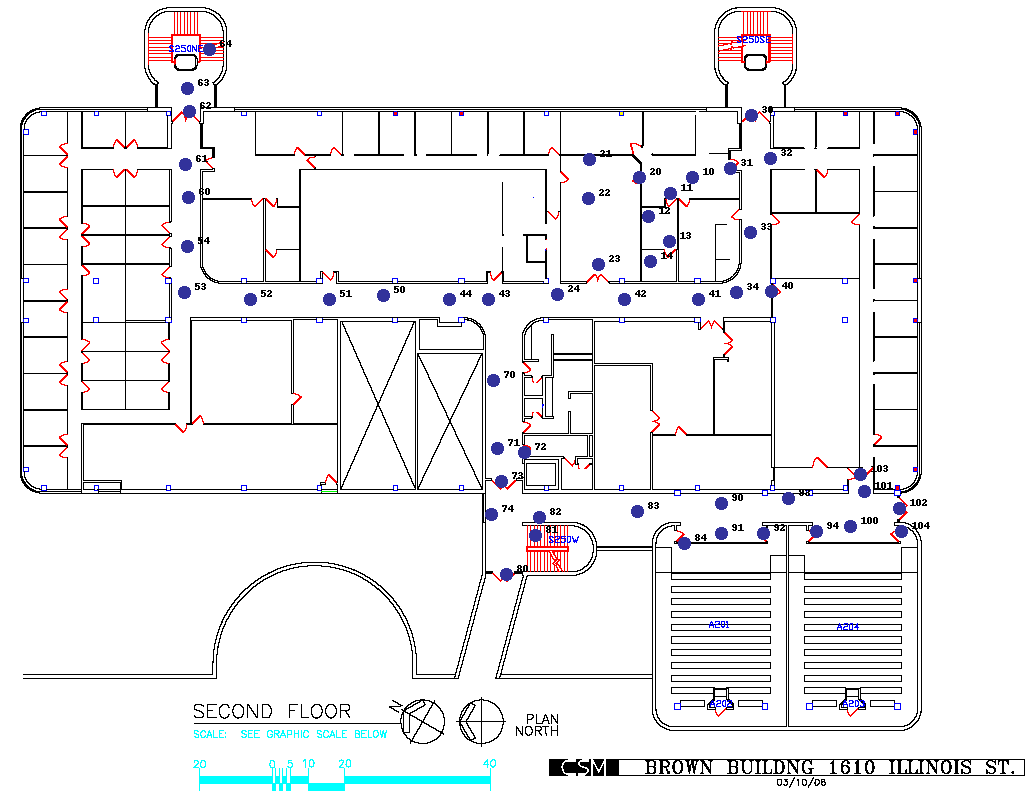
\includegraphics[width=.8\linewidth]{bb_floor2_sensors_old.png}
  \caption{Colorado School of Mines Brown building second floor}
  \label{fig:sub1}
\end{subfigure}
\begin{subfigure}{.45\textwidth}
  \centering
  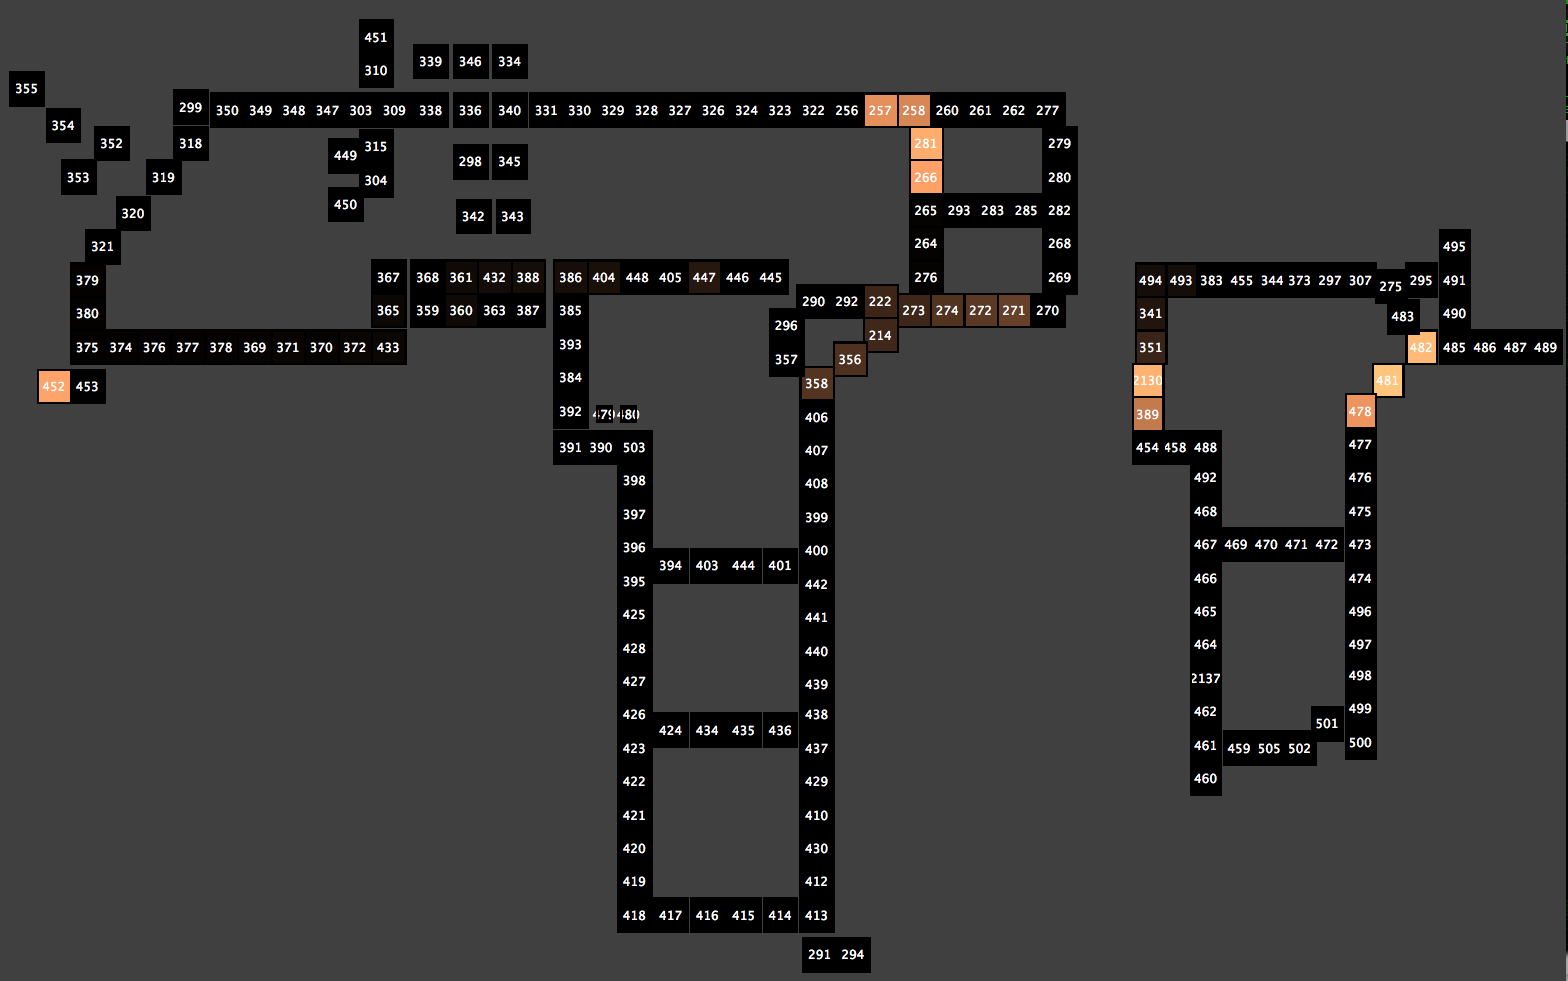
\includegraphics[width=.8\linewidth]{merl_map.png}
  \caption{Merl research lab 7th and 8th floor}
  \label{fig:sub2}
\end{subfigure}
\caption{Sensor locations for buildings}
\label{fig:test}
\end{figure*}


\section{Occupancy Data}
 
Our datasets come from two sources.  The first is a combined research and office building from Mitsubishi's MERL dataset \cite{Wren2007}.  The second is a classroom and office building from the Colorado School of Mines Brown Building (CITE OUR PRIOR WORK).  Both datasets use passive infrared sensors to estimate motion in an area.  We use this data as our occupancy estimation.  To handle instances where an individual may stand under a sensor for an extended period of time thus creating multiple readings when only one is necessary, we first remove the largest outliers from our datasets as defined by the standard deviation of the counts of people at that time.

\subsection{Misubishi's Dataset} 

The Mitsubishi's electronic research labs dataset (MERL) a collection of over 200 passive infrared sensors place densely throughout the 7th and 8th floor of a research office building.  The sensors sensors are place roughly two meters apart on the ceilings creating a dense sensing area with little non-sensed space.  Readings are taken at the milisecond level, but due to the sensors settling times the interdetection time of motion is approximately 1.5 seconds.  

The data was collected from March 2006 through March 2008 and there are roughly 53 million sensor readings.  This building similar to most office buildings with a number of personal offices along with labs and conference rooms.  Employees have roughly set schedules and holdiays are observed as normal. 

The counts of sensor activations have been aggregated every 10 minutes.  Because of the lack of significant motion in the night, we look only at activations that occur between 6:00am and 7:00pm daily.  A plot of the average activations of all Wednesdays for a single sensor along with a range of one standard deviation is given in figure~\ref{fig:merlday}.  Peak motion unsurprisingly occurs during the middle of the day corresponding to lunch time.  There is another small peak of motion near the start of the day corresponding to people entering.  Near the end of the day, instead of a peak there is a region corresponding to high variance.  This seems to imply that while people enter at roughly the same time, there is a significant variance on when people leave the building.

\subsection{Colorado School of Mines Dataset}

The Colorado School of Mines dataset (CSMBB) is a collection of 50 passive infrared sensors mounted on the ceiling of the second floor a class and office room building.  The density of the sensor placement depends on the location within the building.  Outside auditorium is a dense collection of sensors place every meter.  Throughout the rest of the building the sensors are placed roughly every 5 meters.  Data was collected for one academic school year 2008 to 2009.  To acquire readings, the sensors were polled every second and recorded data if motion was detected.  

\begin{figure}[h]
\centering
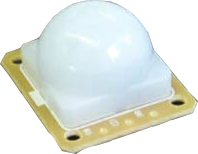
\includegraphics[width = .4\linewidth]{pir_sensor.png}
\caption{Passive infrared motion detector}
\end{figure}

This building operates much differently than the MERL dataset as classes provide motion on a rigid schedule during the day.  Also as students have exams and projects, late night motion is sporadic based on the time of year.    The counts of sensor activations have been aggregated every 10 minutes.  Despite occasional late night motion during exam time, most nights have no significant motion.  For this reason we only collect data between 7:00am and 7:00pm daily.  A plot of the average activations of all Wednesdays for a single sensor along with a range of one standard deviation is given in figure~\ref{fig:csmday}.  The defined peaks in the dataset correlate to class start and end times when most students will be in the hallways of the building.

\begin{figure*}[t!]
\centering
\begin{subfigure}{.45\textwidth}
  \centering
  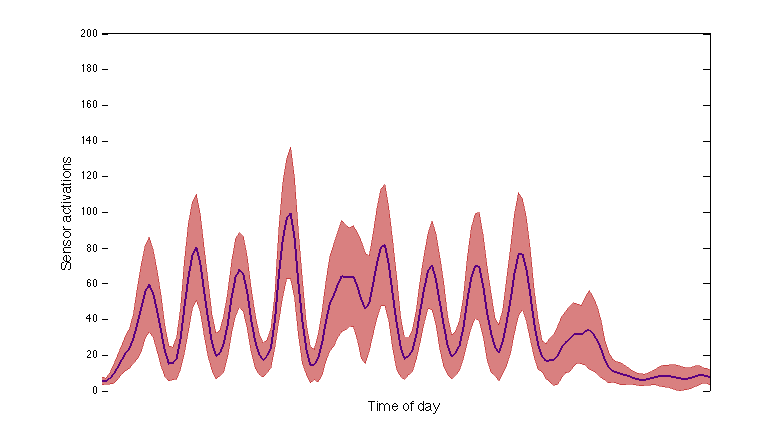
\includegraphics[width=1.0\linewidth]{brown_day.png}
  \caption{CSM Brown Building typical day}
  \label{fig:csmday}
\end{subfigure}
\begin{subfigure}{.45\textwidth}
  \centering
  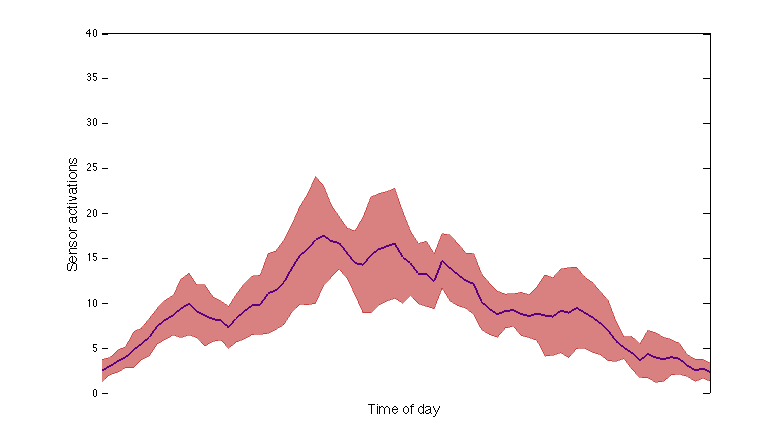
\includegraphics[width=1.0\linewidth]{merl_day.png}
  \caption{MERL typical day}
  \label{fig:merlday}
\end{subfigure}
\caption{Average sensor activations for a specific sensor on Wednesdays with one standard deviation range}
\label{fig:dayplot}
\end{figure*}


\section{Forecasting models}
For comparison we select from some of the most common models used for time series forecasting.  This section gives a brief introduction to each of these forecasting models. 

As an introduction to some notation used for these models we define the time series dataset as $\{T_{t}^{(m)}\}$ data used for these models comes from a set of $M$ binary infrared sensors.  Each $T_{t}^{m}$ is a 10 minute aggregate of sensor $m$ reading at time block $t$.  

\subsection{Seasonal ARIMA Model}
The Auto Regressive Moving Average Model (ARMA) or derivations on its form (Auto regressive integrated moving average, Seasonal auto regressive moving average, etc) have been used in numerous forecasting applications from economics to vehicle traffic systems.  While we have been unable to find ARMA based models used on building occupancy data directly, we have found it used to forecast building energy usage and vehicle occupancy \cite{Williams2003, Hong2011, Newsham2010}.  Its forecasting accuracy is quite strong it can serve as a strong baseline of comparison for a forecasting problem.  

Due to our traffic data having periodic trends and a non stationary mean, a seasonal ARIMA model is best suited to fit our data from the class of ARMA models.  The seasonal ARIMA model is defined as:
\begin{equation}
\label{eq:sarima}
\phi_{p}(B)\Phi_{p}(B^{s})\nabla^{d}\nabla^{D}_{s}T_{t} = \theta_{q}(B)\Theta_{Q}(B^{s})e_{t}
\end{equation}

\noindent
where $\{T_{t}\}$ is our observed time series and $\{e_t\}$ represents an unobserved white noise series ($e_{t} \sim N(0, \sigma^{2})$ )the values of which are computed through model training and are not known a priori.  $B$ is the backshift operator which is a function that allows access to older time readings.  For example $BT_{t} = T_{t-1}$ and $B^{5}T_{t} = T_{t-5}$.  $\nabla^{D}_{s}$ is the seasonal difference operator ($\nabla^{D}_{s}T_{t} = (1 - B^{s})^{D}T_{t}$)and $\phi,\  \Phi,\  \theta,\ \Theta$ are trainable parameters.  

Seasonal ARIMA models are defined as \newline ARIMA(p,d,q)(P,D,Q)$_{s}$ where p is the number of autoregressive terms, d is the number of differences and q is the number of moving average terms.  P, D, and Q all correspond to the seasonal equivalents of p, d, and q.  The parameter $s$ is the seasonality of the model.  For a full discussion of seasonal ARIMA models see Box and Jenkins \cite{Box2008}. \newline

Finding the correct values of $p, d, q, P, D, Q, s$ is traditionally a hard problem.  For a full discussion of finding the correct parameter values applied to a forecasting problem see Williams \cite{Williams2003}.  As a verification of our model, we applied the LJung-Box test \cite{Ljung1978} on our set of residual data for each model. Both residual sets passed: $p = 0.9964$ MERL and $p = 0.1072$ CSMBB.  Our final model parameters can be seen in the table below.  Notice that the season is different for each model due to a difference in window of time for each day that we extracted data.

\begin{center}
\begin{tabular}{|c|c|c|c|c|c|c|c|} \hline
Dataset & p & d & q & P & D & Q & s\\ \hline
MERL & 0 & 0 & 1 & 0 & 1 & 5 & 78\\ \hline
CSMBB & 0 & 1 & 1 & 0 & 1 & 3 & 72\\ \hline
\end{tabular}
\end{center}

Forecasting from this model is performed by iteratively forward feeding values of the model into itself.  Since the set of residuals $e$ from a properly trained seasonal ARIMA model is described by a white noise gaussian distribution $N(0, \sigma^{2})$ , we can take the expected value of the residual at time $e_{t + 1}$ to be 0.  This leaves us with the following forecasting equation: 

\begin{equation}
\label{eq:sarima}
\phi_{p}(B)\Phi_{p}(B^{s})\nabla^{d}\nabla^{D}_{s}T_{t + 1} = \theta_{q - 1}(B)\Theta_{Q - 1}(B^{s})e_{t}
\end{equation}

\subsection{Historic Average}
This model is simply the per day average of readings at each time step.  For certain types of data this model is has been shown to be more accurate than seasonal ARIMA forecasting \cite{Newsham2010}, specifically when the data has a strong historic correlation.  Average forecasts have the advantage of being extremely computationally fast and having a forecast accuracy that does not depend on the forecasting horizon.  This result will be shown later.


\subsection{Time Delayed Neural Networks}

\begin{figure*}[t!]
\centering
\begin{subfigure}{.45\textwidth}
  \centering
  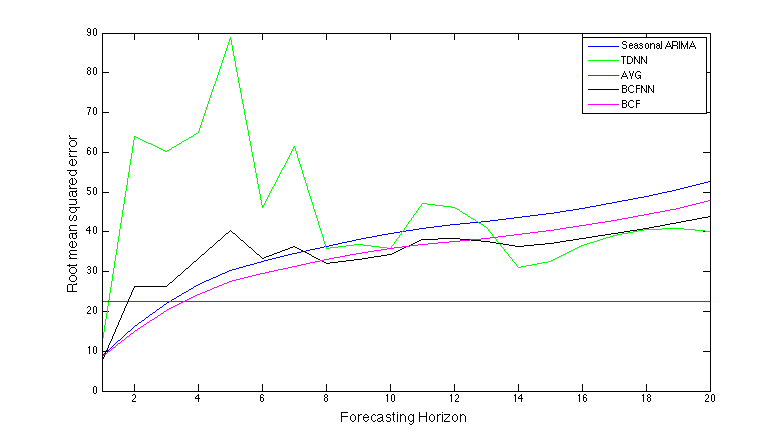
\includegraphics[width=1.0\linewidth]{rmse_brown.png}
  \caption{CSMBB forecasting model errors}
  \label{fig:csmrmse}
\end{subfigure}
\begin{subfigure}{.45\textwidth}
  \centering
  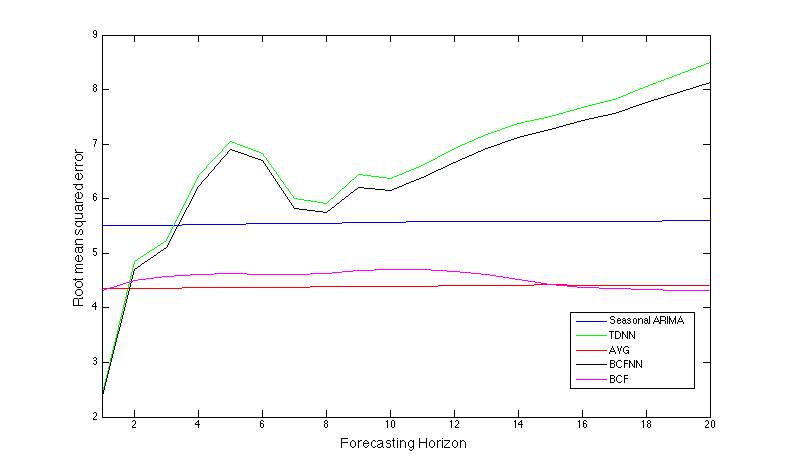
\includegraphics[width=1.0\linewidth]{rmse_merl.png}
  \caption{MERL forecasting model errors}
  \label{fig:merlrmse}
\end{subfigure}
\caption{Root mean square error of forecasting for each model vs forecasting horizon}
\label{fig:rmseplot}
\end{figure*}

\begin{figure}[ht!]
\centering
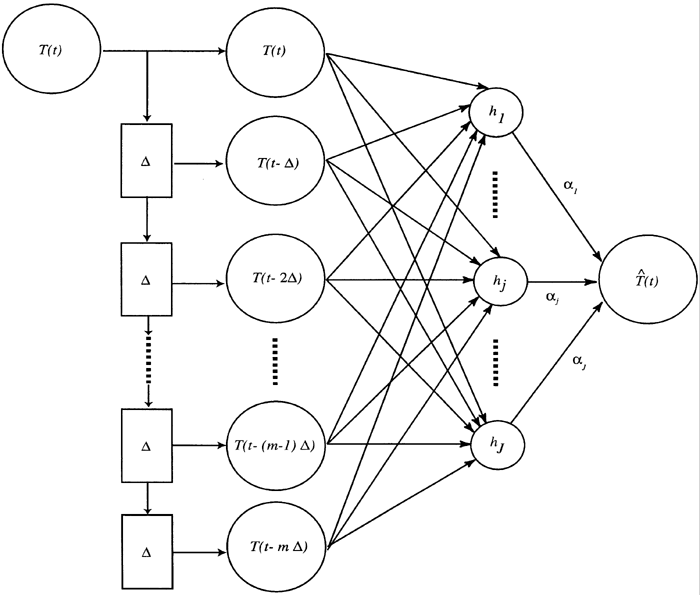
\includegraphics[width = .8\linewidth]{time_delay_neural_network.png}
\caption{Architecture of a time delayed neural network with $m + 1$ inputs and $\bf{J}$ outputs \cite{Hansen2003}.}
\end{figure}

Time delayed neural networks are a special subset of regression neural networks where the input data is a local history of data from the time series.  Commonly the output is a single point forecast from that same time series at some point $t + \delta$ in the future.   The form of our 1 hidden layer time delayed neural network is:

\begin{equation}
T_{t + 1} = \phi \{ \sum_{j = 1}^{J} w_{j}\psi_{j} \bigg[ \sum_{l = 0}^{m}w_{ji}T_{t - l\delta} + w_{j0} \bigg] + w_0 \}
\end{equation}

\noindent where $\phi()$ is a linear activation function on the output layer and $\psi()$ is the standard sigmoid function.

Forecasting is performed by computing the output for a $m + 1$ length window of time and then iteratively forecasting a set of time steps in the future by using forecast data as inputs into the next forecast. 

\subsection{Bayesian Combined Forecasting}

The Bayesian combined forecasting (BCF) approach is one of several types of approaches which attempt to combine several forecasting methods.  The approach works by computing a normalized likelihood for each forecasting model's accuracy of forecast at that point in time in the dataset.  For example if we are performing a combined forecast on a seasonal ARIMA model and a time delayed neural network model then at each forecast point $t$ we compute the likelihood of each model's prediction at that point in time.  From this set of likelihood we can then perform a final prediction for $t + \delta$.

A full description of the model is done by Petridis \cite{Petridis2001}.  The final forecasting equation is given by:

\begin{equation}
\label{eq:model_prob}
p_{t}^{k} = p(k|T_{1:t}) = \frac{p_{t - 1}^{K} \cdot e(T_{t} - \bar{T}_{1:t-1}^{k})}{\sum_{j=1}^{K}p_{t - 1}^{j} \cdot e(T_{t}^{j} - \bar{T}_{1:t-1}^{j})}
\end{equation}

\noindent
where $p(k|T_{1:t})$ is the probability of model $k$ given data $T_{t}$, $K$ is the total number of models, $\bar{T}_{t}^{k}$ is the forecast from model $k$, and $e()$ is the probability mass function (PMF) of the forecasting error for model $k$.  

For this work we assume our PMF to be a constant variance white noise gaussian trained for each model.  For future work, we plan to incorporate a more realistic error function based on the changing variance in our forecasting functions and the data.  One such approach would be to use a generalize autoregressive conditional heteroskedastic to forecast what future forecasting variance will be for each model based on local conditions.  We have not yet implemented this and instead simply have a constant gaussian PMF for each model similar to the work done by Zheng \cite{Zheng2006} on traffic forecasting using Bayesian Combined prediction. 

Forecasting using a BCF approach is done by either computing a weighted forecast $\delta$ time steps into the future for each forecasting model or by simply selecting the model with the highest likelihood.  For this paper we forecast using a weighted forecast of all models.  
\begin{equation}
T_{t + \delta} = \sum_{k=1}^{K}p_{t}^{k} \cdot \bar{T}_{t + \delta}^{k}
\end{equation}

Because the Bayesian combined forecasting approach is iterative It is possible that a long section of forecasts that indicate one model correct or incorrect can lead to likelihood underflow.  Due to this problem we adjust our normalized likelihoods so that no model may reach a value below 0.001.  This empirically chosen value has seemed low enough to not have a great impact on forecasts while still being high enough to allow model likelihoods to change quickly.


\begin{figure*}[t!]
\centering
\begin{subfigure}{.45\textwidth}
  \centering
  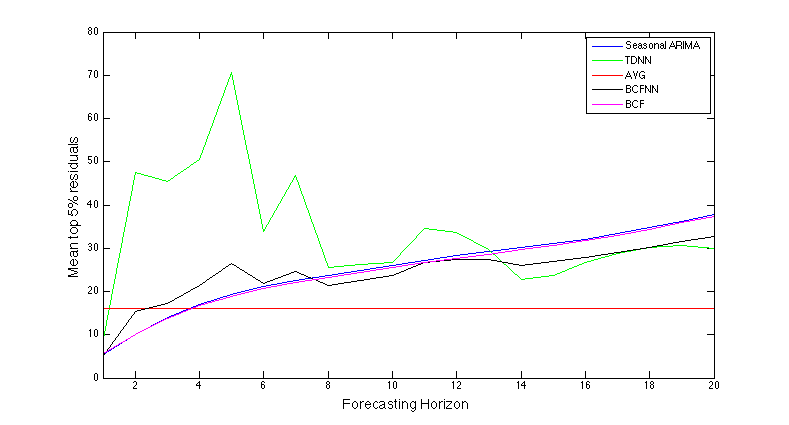
\includegraphics[width=1.0\linewidth]{brown_top5.png}
  \caption{CSMBB top 5\% miss-forecasts}
  \label{fig:csmtop5}
\end{subfigure}
\begin{subfigure}{.45\textwidth}
  \centering
  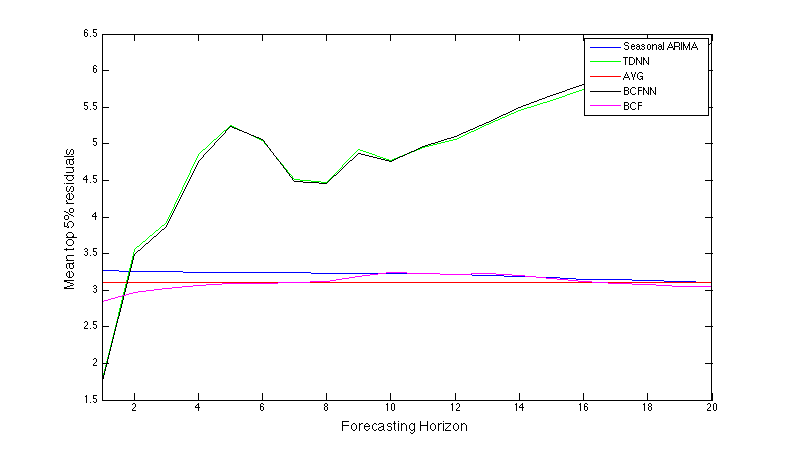
\includegraphics[width=1.0\linewidth]{merl_top5.png}
  \caption{MERL top 5\% miss-forecasts}
  \label{fig:merltop5}
\end{subfigure}
\caption{Average root mean square of the top 5\% of miss-forecasts}
\label{fig:top5plot}
\end{figure*}

One other note on BCF comes from Diebold \cite{Diebold1991} who cautions use of forecasting using a Bayesian combination of models in all cases.  Diebold points out that under certain situations a convex combination of forecasts for models may not be optimal and cases exist where taking negative likelihood weighting may be optimal.  He mentions that these conditions are likely to arise during instances where the data may not be accurately described by any of the forecasting models.  Searching for such situations is beyond the scope of our work and will be saved for later work.  However because our forecasting models were all trained on the same datasets, if such a situation arose, each individual dataset would suffer from the same forecasting problem. 

\section{Results}

Here we give the results of implementations for each of our models on each dataset.  All of these results are run on the same set of models as described above.  With the only exception being two different versions of a BCF.  BCFNN is a Bayesian combined forecaster with an average model, a seasonal ARIMA model and a TDNN model, while BCF is simply a Bayesian combined forecaster without a TDNN model.  This comparison was performed due to the TDNN model having a significant affect on the performance of the BCF.

All of the models were trained on 60\% of the total datasets.  Another 20\% was used for model validation the final 20\% used for testing.  All results that follow are on the test set only.

\subsection{Data metrics}

\subsection{Discussion of results}
Figure~\ref{fig:rmseplot} shows the results of the root mean squared error of forecasts across a forecast horizon up to 20 time steps (200 minutes) into the future for each model.  The average model shows itself to be a strong indicator of future activity for forecasts beyond 30 minutes into the future.   In the CSMBB dataset the Seasonal ARIMA model was a good forecaster of future activity while in the MERL set is performed significantly worse than even the average model on all forecasting horizons.  This is likely due to a stronger seasonal component to the CSMBB dataset due class schedules.  Instead on the MERL dataset there is little seasonal correlation and thus natural variance from a prior season may incorrectly affect current forecasts.

The BCFNN and BCF forecasting models always performed better the worst component model and in general seems to offer an improvement in forecasting accuracy.  In general the BCFNN models follow the TDNN model.  This is likely due to the model's strong short term forecasting accuracy which effects the likelihood of that model forecasting $\delta$ steps in the future.

\section{Conclusion}

\begin{figure*}[t!]
\centering
\begin{subfigure}{.45\textwidth}
  \centering
  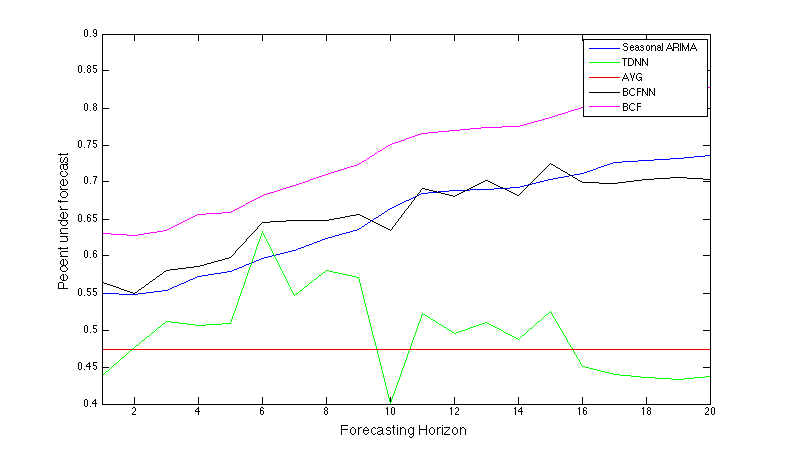
\includegraphics[width=1.0\linewidth]{brown_ou.png}
  \caption{CSMBB forecasts under actual data}
  \label{fig:csmou}
\end{subfigure}
\begin{subfigure}{.45\textwidth}
  \centering
  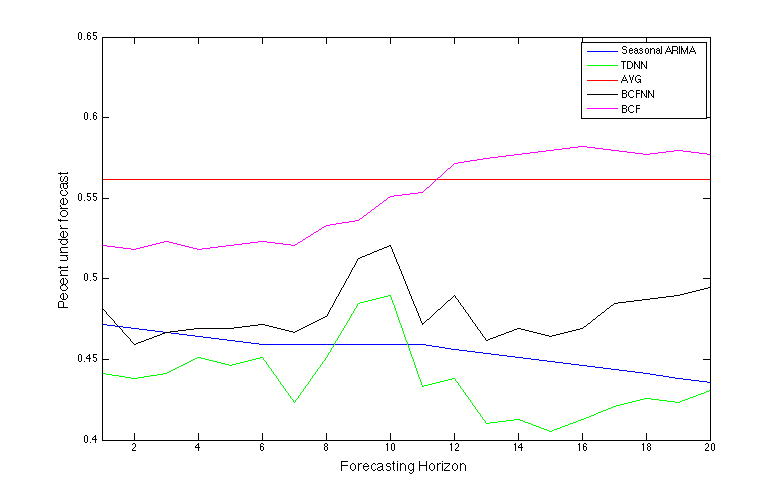
\includegraphics[width=1.0\linewidth]{merl_ou.png}
  \caption{MERL forecasts under actual data}
  \label{fig:merlou}
\end{subfigure}
\caption{Percent of forecasts under the actual data per model vs forecast horizon}
\label{fig:ouplot}
\end{figure*}

\bibliographystyle{abbrv}
\bibliography{big-data_mining} 
\balancecolumns

\end{document}
